\documentclass[letterpaper,12pt]{article}
\usepackage{array}
\usepackage{threeparttable}
\usepackage{geometry}
\geometry{letterpaper,tmargin=1in,bmargin=1in,lmargin=1.25in,rmargin=1.25in}
\usepackage{fancyhdr,lastpage}
\pagestyle{fancy}
\lhead{}
\chead{}
\rhead{}
\lfoot{}
\cfoot{}
\rfoot{\footnotesize\textsl{Page \thepage\ of \pageref{LastPage}}}
\renewcommand\headrulewidth{0pt}
\renewcommand\footrulewidth{0pt}
\usepackage[format=hang,font=normalsize,labelfont=bf]{caption}
\usepackage{listings}
\lstset{frame=single,
  language=Python,
  showstringspaces=false,
  columns=flexible,
  basicstyle={\small\ttfamily},
  numbers=none,
  breaklines=true,
  breakatwhitespace=true
  tabsize=3
}
\usepackage{amsmath}
\usepackage{amssymb}
\usepackage{amsthm}
\usepackage{harvard}
\usepackage{setspace}
\usepackage{float,color}
\usepackage[pdftex]{graphicx}
\usepackage{hyperref}
\hypersetup{colorlinks,linkcolor=red,urlcolor=blue}
\theoremstyle{definition}
\newtheorem{theorem}{Theorem}
\newtheorem{acknowledgement}[theorem]{Acknowledgement}
\newtheorem{algorithm}[theorem]{Algorithm}
\newtheorem{axiom}[theorem]{Axiom}
\newtheorem{case}[theorem]{Case}
\newtheorem{claim}[theorem]{Claim}
\newtheorem{conclusion}[theorem]{Conclusion}
\newtheorem{condition}[theorem]{Condition}
\newtheorem{conjecture}[theorem]{Conjecture}
\newtheorem{corollary}[theorem]{Corollary}
\newtheorem{criterion}[theorem]{Criterion}
\newtheorem{definition}[theorem]{Definition}
\newtheorem{derivation}{Derivation} % Number derivations on their own
\newtheorem{example}[theorem]{Example}
\newtheorem{exercise}[theorem]{Exercise}
\newtheorem{lemma}[theorem]{Lemma}
\newtheorem{notation}[theorem]{Notation}
\newtheorem{problem}[theorem]{Problem}
\newtheorem{proposition}{Proposition} % Number propositions on their own
\newtheorem{remark}[theorem]{Remark}
\newtheorem{solution}[theorem]{Solution}
\newtheorem{summary}[theorem]{Summary}
%\numberwithin{equation}{section}
\bibliographystyle{aer}
\newcommand\ve{\varepsilon}
\newcommand\boldline{\arrayrulewidth{1pt}\hline}


\begin{document}

\begin{flushleft}
  \textbf{\large{Problem Set \#3}} \\
  MACS 30000, Dr. Evans \\
  Cheng Yee Lim
\end{flushleft}

\vspace{5mm}

\noindent\textbf{Problem 1}\\
\begin{figure}[htb]\centering\captionsetup{width=4.0in}
  \caption{\textbf{Scatter plot of lifetime temperature of Ricardo}}\label{FigExample}
  \fbox{\resizebox{6.0in}{4.0in}{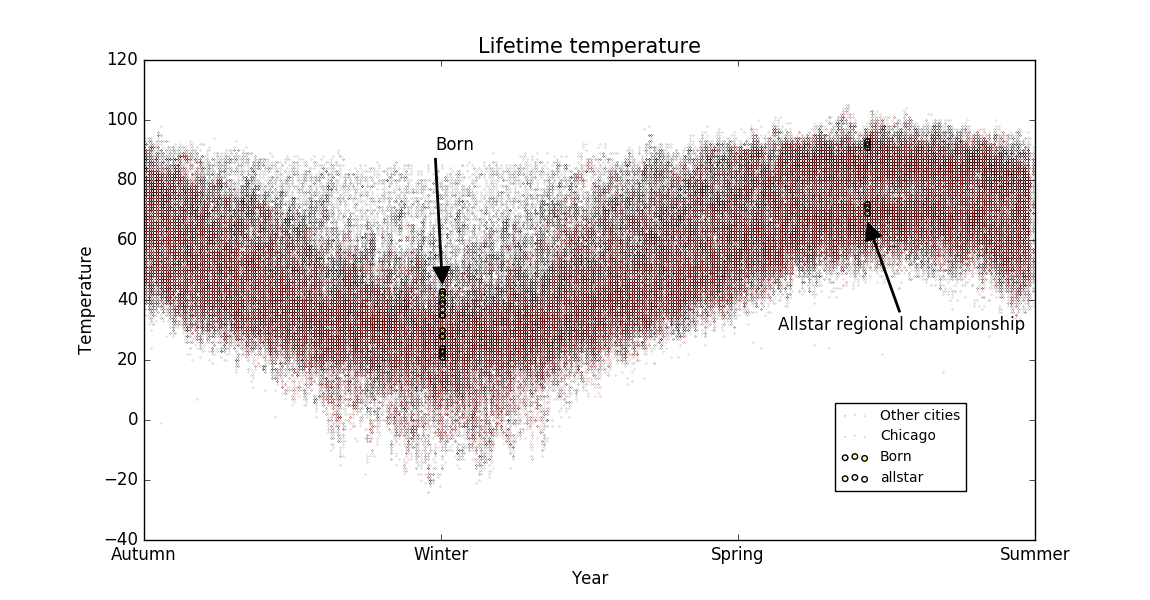
\includegraphics{images/Q1scatter.png}}}
\end{figure}
\flushleft
\textbf{Part (a).}
\flushleft Using the datetime function, I created a new index that corresponds to the month and day of a date separately for leap years and non-leap years i.e. the index starts at 265 and ends at 630 for leap years and starts at 264, and ends at 628 for non-leap years. This would allow us to plot the x-axis as one complete year, with several years of months and dates.
\flushleft

\textbf{Part (b).} \\
\flushleft I then merged the high and low temperature of cities by appending the axes to form a dataframe of all temperatures for its corresponding monthday. This dataframe was used as the y variable of the scatter plot. 
\flushleft

\textbf{Part (c).} \\
\flushleft I set my marker color as black and size as s=0.01 for the general markers.
\flushleft

\textbf{Part (d).} \\
\flushleft I set my marker color as maroon and size as s=0.01 for the Ricardo's Illinois markers.
\flushleft

\textbf{Part (e).} \\
\flushleft I highlighted life events of "born" and "little league all-star team wins regional championship" by setting the marker color as yellow, and adding a black bold border around the marker. Using the annotate function, I then labeled these datapoints with descriptive text. 
\flushleft

\textbf{Part (f).} \\
\flushleft I then labeled the x-axis evenly spaced as 'Autumn', 'Winter', 'Spring', 'Summer'. The y-axis was labeled as temperature. 
\flushleft

\newpage
\noindent\textbf{Problem 2}\\
\textbf{Part (a).} \\
\begin{figure}[htb]\centering\captionsetup{width=4.0in}
  \caption{\textbf{2D frequency histogram of concentration of plasma cholesterol (mg/dl)}}\label{FigExample}
  \fbox{\resizebox{4.0in}{3.0in}{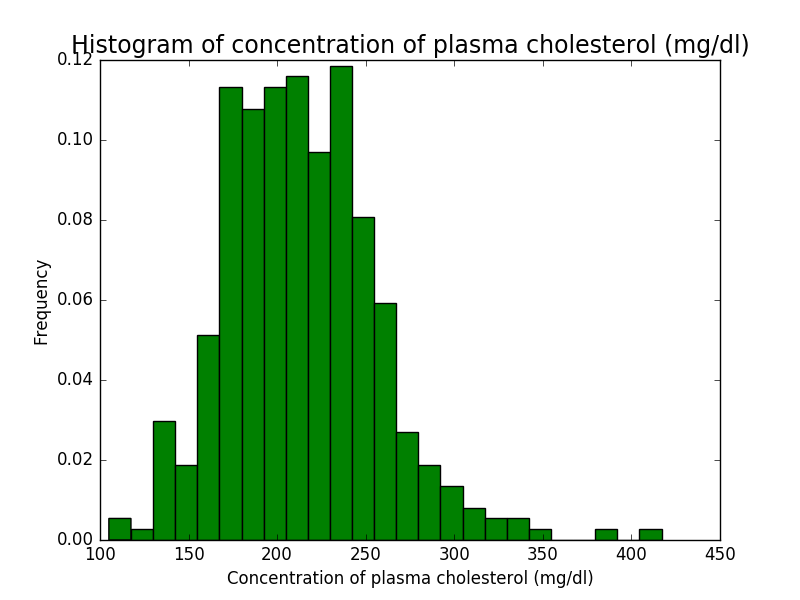
\includegraphics{images/chol_hist_2a.png}}}
\end{figure}

\flushleft I extracted the information on concentration of plasma cholesterol from the lipids.csv file and plotted a 2D frequency histogram with 25 equally spaced bins. The midpoint of the bin with the highest frequency is 237.50. \\
\newpage
\textbf{Part (b).} \\
\begin{figure}[htb]\centering\captionsetup{width=4.0in}
  \caption{\textbf{3D frequency histogram of concentration of plasma triglycerides (mg/dl) and cholesterol (mg/dl)}}\label{FigExample}
  \fbox{\resizebox{4.0in}{3.0in}{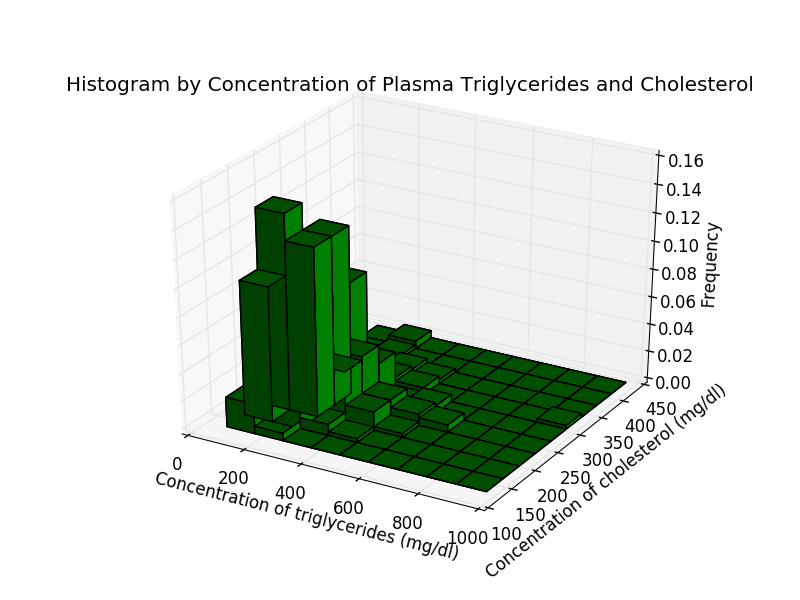
\includegraphics{images/3d_hist_2b.png}}}
\end{figure}
\flushleft The key new finding that emerged from the data is that individuals who have low concentration of plasma triglycerides are more likely to have low concentration of plasma cholesterol. However, individuals generally have higher concentration of plasma cholesterol than plasma triglycerides. \\

\textbf{Part (c).} \\
\flushleft Individuals with concentration of plasma triglycerides and plasma cholesterol of higher than 300mg/dl have the highest risk for heart disease.\\

\newpage
\noindent\textbf{Problem 3}\\
\begin{figure}[htb]\centering\captionsetup{width=4.0in}
  \caption{\textbf{Normalized peak plot of job growth in the past 14 recessions in the US}}\label{FigExample}
  \fbox{\resizebox{6.0in}{4.0in}{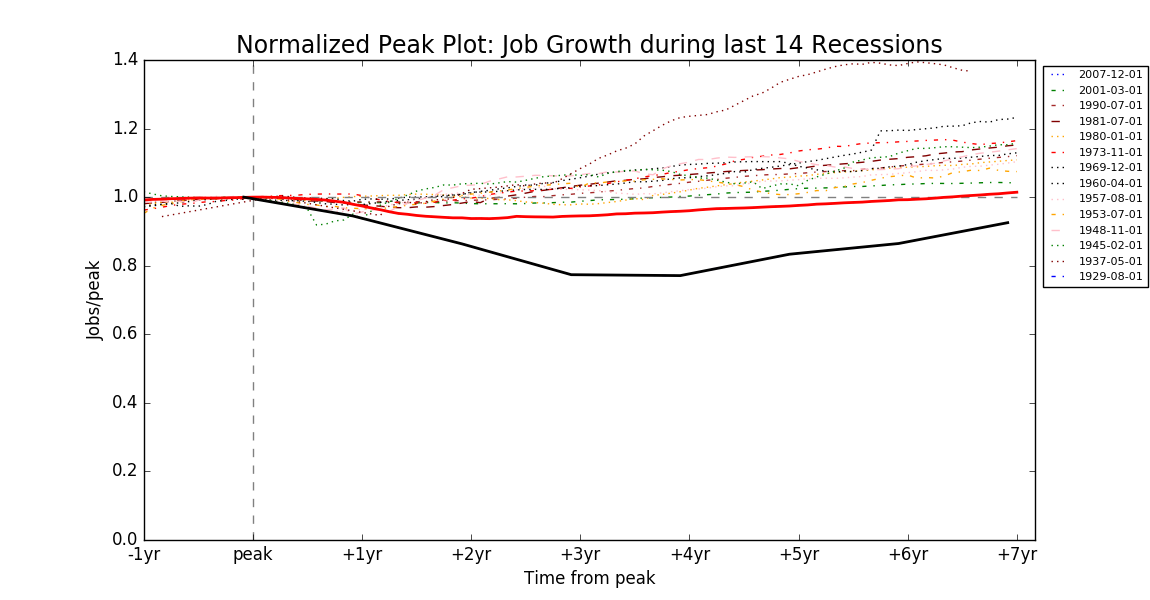
\includegraphics{images/recessions.png}}}
\end{figure}

\textbf{Part (a).}
\flushleft I created 14 segments of job growth data series by selecting the dates in the indexes for 14 recessions since 1929.
\flushleft

\textbf{Part (b).}
\flushleft I normalized each of the 14 series such that the jobs level at the peak date equals to 1.
\flushleft

\textbf{Part (c)(d)(e)(f)(g)}
\flushleft The 14 series were plotted as a line graph with normalized jobs against time from the peak to show the percent change from the peak jobs level. Each line plot has a different combination of linestyle and color and a legend is made outside of the axis on the right that states the beginning date of each recession. The y-axis is then labelled as "Jobs/Peak" and the x-axis is labelled as "Time from Peak", with 9 markers:  -1yr, Peak, +1yr, +2yr, +3yr, +4yr, +5yr, +6yr, +7yr. 
\newpage
\textbf{Part (h).}
\flushleft A dashed grey horizontal line at Jobs/Peak =1 and a dashed grey vertical line at Peak were drawn, to act as a reference point in interpreting the graph.
\flushleft

\textbf{Part (i).}
\flushleft The line plot for the Great Depression is black and solid and the line plot for the Great Recession is red and solid. The line plots are also thicker than the other 12 plots.
\flushleft

\textbf{Part (j).}
\flushleft The recession in 1945 February was worse than the Great Recession in terms of the percent of jobs loss, but the recession in 1945 February experienced a much faster job recovery rate.
\flushleft

\textbf{Part (k).}
\flushleft There are no ways in which the Great Recession has been worse than the Great Depression in the United States, in terms of jobs losses.
\flushleft


\end{document}
